\documentclass[mathserif,serif]{beamer}
\usepackage[utf8]{inputenc}
\usepackage[english]{babel}
\usepackage{amsmath}
\usepackage{stmaryrd}
\usepackage{amsfonts}
\usepackage{amssymb}
\usepackage{hyperref}
\usepackage{graphicx}
\usepackage{url}
\usepackage{amsthm}
\usepackage{mathpartir}
\usetheme{Warsaw}

\begin{document}

\newtheorem{proposition}{Proposition}
\setbeamertemplate{theorems}[numbered]

\author[Di Giacomo]
{Francesco ~Di Giacomo}
\institute[Universities Here and There] % (optional)
{
  Università Ca' Foscari di Venezia - PhD in Computer Science
}
\date{}
\title{Building Domain Specific Languages with the Metacasanova meta-compiler}

\frame{\titlepage}

\begin{frame}
	\frametitle{Introduction}
	\framesubtitle{Importance of domain specific languages}
	\begin{itemize}
		\item They allow to express the solution of a problem in a more natural way.
		\item They provide constructs that are domain-specific not provided by GPL's.
		\item They allow to develop complete application programs for a specific domain more quickly.
	\end{itemize}
	
	\pause
	\textbf{CONSEQUENCE:} It is desirable to deploy a DSL's when the scope of the application is very specific.
	
\end{frame}

\begin{frame}
	\frametitle{Introduction}
	\framesubtitle{Some DSL's examples}
	
	\begin{figure}
		\centering
		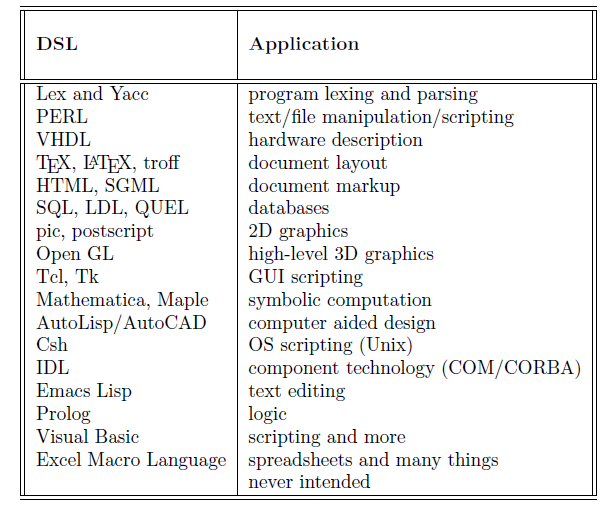
\includegraphics[scale=0.5]{Figures/dsl_table}
	\end{figure}	
\end{frame}

\begin{frame}
	\frametitle{Introduction}
	\framesubtitle{Disadvantages of DSL's}
	
	\textbf{PROBLEM}: Creating DSL's requires to implement a compiler/interpreter for the language.
	
	\begin{itemize}
		\item Compilers are complex
		\item Several modules: parser, type checker, code generator/code interpreter
		\item Require a lot of development time.
		\item Not flexible: adding features to the language compiled by hard-coded compilers takes a considerable effort.
	\end{itemize}
\end{frame}

\begin{frame}
	\frametitle{Towards meta-compilers}
	\framesubtitle{Implementing compilers is repetitive}
	
	The implementation of the compiler is a repetitive process:
	\begin{itemize}
		\item The parser can be created with parser generators (e.g. Yacc)
		\item The type system must be implemented in the host language.
		\item The operational semantics must be reflected in the generated code (code generations).
	\end{itemize}
\end{frame}

\begin{frame}
	\frametitle{Towards meta-compilers}
	\framesubtitle{Type system and semantics}
	
	How they are formalized:
	\begin{itemize}
		\item Expressed in a form that mimics logical rules.
		\item They are compact.
		\item They are readable.
	\end{itemize}
	
	How they are implemented:
	\begin{itemize}
		\item Encoded with the abstractions provided by the host language.
		\item Readability is usually lost in the translation process.
		\item The effort required for the translation is high.
	\end{itemize}
	
\end{frame}

\begin{frame}
	\frametitle{Towards meta-compilers}
	\framesubtitle{Example of semantics}
	
	Semantics of a statement that waits ford a condition or a certain amount of seconds:
	
	\vspace{0.5cm}
	\small
	\inferrule
	{\langle t - dt > 0 \rangle \; \Rightarrow \; \texttt{true}}
	{\langle \mathtt{wait} \; t;k \; dt \rangle \; \Rightarrow \; \langle \mathtt{wait} \; t - dt ; k \; dt \rangle}
	
	\inferrule
	{\langle t - dt > 0 \rangle \; \Rightarrow \; \texttt{false}}
	{\langle \mathtt{wait} \; t ; k \; dt \rangle \; \Rightarrow \; \langle k \; dt \rangle}
	
	\small
	\inferrule
	{\langle c \rangle \; \Rightarrow \; \mathtt{true}}
	{\langle \mathtt{wait} \; c;k \; dt \rangle \; \Rightarrow \; \langle k \; dt\rangle}
	
	\inferrule
	{\langle c \rangle \; \Rightarrow \; \mathtt{false}}
	{\langle \mathtt{wait} \; c;k \; dt \rangle \; \Rightarrow \; \langle \mathtt{wait} \; c;k \; dt \rangle}
\end{frame}

\begin{frame}
		\frametitle{Towards meta-compilers}
		\framesubtitle{Implementation}
		
		**STUB**
		Paste the code for wait state machine from Casanova compiler
\end{frame}

\end{document}